\documentclass{Resources/netsci-project}

% :::~ This is the configuration for the bibliography. DO NOT CHANGE
\usepackage[
    backend=biber,
    style=authoryear,
    natbib=false,
    maxcitenames=2,
    minbibnames=1, maxbibnames=99, 
    url=false, 
    doi=true,
    ]{biblatex}
\addbibresource{references.bib}
\usepackage{verbatim}
\usepackage{hyperref}

\begin{document}
\firstpage{1}
\subjectarea{Blockchain \& Distributed Ledger Technologies}
\title{Final Project - Epidemic spreads over the flight network}
\author{Marlene Funke (15-738-719), Aleksandar Novković (16-733-032), Sandra Trachsel (15-718-190), Miguel Vázquez (16-712-598)}
\course{Network Science}
\school{Faculty of Business, Economics and Informatics}
\date{December 19th, 2022}
\maketitle

%%%%%%%%%%%%%%%%%%%%%%%%%%%%%%%%%%%%%%%%%%%%%%%%%%%%%%%%%%%%%%%%%%%%
%%%%%%%%% ABSTRACT
%%%%%%%%%%%%%%%%%%%%%%%%%%%%%%%%%%%%%%%%%%%%%%%%%%%%%%%%%%%%%%%%%%%%

\begin{abstract}
The abstract is a short text.
\end{abstract}

%%%%%%%%%%%%%%%%%%%%%%%%%%%%%%%%%%%%%%%%%%%%%%%%%%%%%%%%%%%%%%%%%%%%
%%%%%%%%% INTRODUCTION
%%%%%%%%%%%%%%%%%%%%%%%%%%%%%%%%%%%%%%%%%%%%%%%%%%%%%%%%%%%%%%%%%%%%

\section{Introduction}
Here we introduce the paper. 
Hypothesis: closeness centrality best measure since it's the one used to identify spreader nodes according to what was seen in the lecture.

%%%%%%%%%%%%%%%%%%%%%%%%%%%%%%%%%%%%%%%%%%%%%%%%%%%%%%%%%%%%%%%%%%%%
%%%%%%%%% THEORY
%%%%%%%%%%%%%%%%%%%%%%%%%%%%%%%%%%%%%%%%%%%%%%%%%%%%%%%%%%%%%%%%%%%%

\section{Theory}
\subsection{Literature}
The rapid spread of the new Coronavirus has caused huge social and economic damage around the world. One of the biggest concerns for pandemics is globalization and the fast and frequent movement of individuals across the world due to the extended flight network. The airline Network has heavily increased the speed and scope of human mobility, and with it, it has created an efficient global transport network for infectious diseases, allowing pandemics to spread more rapidly around the world (\cite{Lawyer2016}). International passengers number increased from 1.67 Billion in 2000 to 2.63 Billion in 2010 and an astonishing 4.56 Billion in 2019 just before the COVID-19 pandemic. In 2020 amid the Corona Pandemic, the number of passengers dropped to 1.81 Billion, which is approximately the level of 2005 (\cite{WorldBank}). \\
\cite{Morse2012} explain that the frequency of new emerging pathogens is also increasing over time. And most of these viruses find an origin in animals and infect humans due to behavioural, socioeconomic and economical changes. 
Only in the last few decades we have witnessed the emergency of HIV, Ebola Virus Disease, SARS, H1N1 influenza, MERS-CoV and other novel zoonotic infections. All of these are affecting people and crossing the geopolitical boundaries of nation-states (\cite{MartinBoland2018}).\\
The simulation studies \cite{Colizza2006}, and \cite{Colizza2007} suggest that the explanatory power for relationships between the topology of the world airline network is found in topological descriptors which characterize epidemic outcomes on network models. \cite{Balcan2009}, and \cite{Brockmann2013} both support this conclusion with observational studies of Influenza; nevertheless, this is also supported by studies of other epidemics like malaria (\cite{Hunag2013}) and dengue fever (\cite{Semanza2014}).\\
The topological structure of the World Airline Network is well characterized. The Network is a scale-free small-world network, with a strong community structure that is imposed by spatial constraints (\cite{Lawyer2016, Barrat2005}). The World Airline Network is divided into three parts: The bottom layer has airports with zero clustering coefficient, which is called the Periphery. The intermediate layer is the Bridge, with the airports that connect remote locations to global hubs, and the top layer is the Core, which shows the connections of the major world economic hubs. Figure \ref{fig:layers} shows that 69.41\% of the airports serve as bridges that connect a heavily interconnected core of the 2.26\% major transportation hubs (72 airports) to peripheral airports and regional population centres (28.33\%). For a passenger to travel between any pair of airports, it needs at most to go through 12 connections. However, on average, 33\% of the routes can be covered with at most three connections (\cite{Verma2014}).
\begin{figure}[!ht]
    \centering
    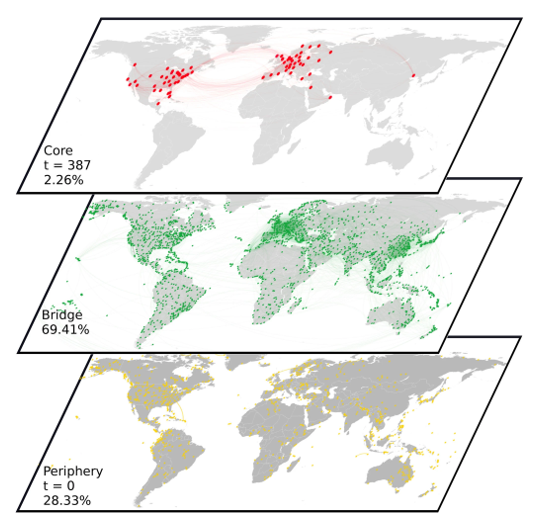
\includegraphics[scale=0.8]{Figures/layers.png}
    \caption{Verma, T., Araújo, N. \& Herrmann, H. Revealing the structure of the world airline network. Sci Rep 4, 5638 (2014). https://doi.org/10.1038/srep05638}
    \label{fig:layers}
\end{figure}
Since actual outcomes of arising infectious diseases are critically shaped by chance events in early stages of their emergence, it is important to understand clearly how seed location can influence global outcomes. This could improve significantly public health planning (\cite{Lawyer2016}). 
This World Airline transportation Network allows us to rationalize the role of its large-scale properties within the predictability and heterogeneity of an epidemic pattern (\cite{Colizza2006TheMO}). 

%%%%%%%%%%%%%%%%%%%%%%%%%%%%%%%%%%%%%%%%%%%%%%%%%%%%%%%%%%%%%%%%%%%%

\subsection{Model assumptions}
To begin with our analysis, we had to make some assumptions. Firstly, we assume that in our network, the nodes represent airports and not people or passengers; additionally, all the airports have the same weight. On the other hand, the edges of our network represent (directed) routes between airports. We weighted those edges by the number of airlines on that route $\times$ the number of seats on the plane type that the airline uses for that route. During our data preparation, we also assumed that the same aircraft models have the same number of seats, and since all flight data was recovered from OpenFlights, we have no reason to believe that they would include cargo-shipping routes in their database. Furthermore, we assume that there is only one flight per route and period.
Furthermore, we also fix the recovery rate at \textcolor{red}{XXX} and the infection rate at \textcolor{red}{XXX}.

A further assumption is that some Regulation exists that allows us to completely shut down any airport and all of its routes and that the selected airports will cancel all their flights at the same time. 
Finally, we assume, that airports that shut down after other airports have been infected \textcolor{red}{(fixed (?) at XXX\%)}. In this way, we can reflect on the delay between the emergence of the virus and the action taken by governments. Moreover, it reduces the likelihood of trivial epidemics, where only the initial randomly infected node(s) are infected by the end as no transmission occurs.


\begin{itemize}
 %   \item wanken
 %   \item Nodes represent airports and not people, and they are all weighted the same
  %  \item Edges represent routes (i.e. directed!) between airports, weights are given by nr of airlines on that route $\times$ number of seats on plane type used by that airline on that route. Further assume, during data preparation, that same models of aircraft have the same number of seats and that all flights we recovered from OpenFlights are airliners carrying passengers as we have no reason to believe they would include cargo-shipping routes in their database
 %  \item One flight per route every period
 %   \item Infection rate is fixed (?) at XXX
 %   \item Recovery rate is fixed (?) at XXX
 %   \item Regulation exists that allows to shut down all routes of any airport in the world. We assume all airports which are selected to be shut down shut down completely and at the same time.
 %   \item Airports are shut-down after already several nodes (fixed (?) at XXX\%) have been infected. This better reflects the delay between the emergence of a virus and action taken by governments. It also reduces the likelihood of trivial epidemics, where only the initial randomly infected node(s) are infected by the end as no transmission occurs.
\end{itemize}


%%%%%%%%%%%%%%%%%%%%%%%%%%%%%%%%%%%%%%%%%%%%%%%%%%%%%%%%%%%%%%%%%%%%
%%%%%%%%% METHODS
%%%%%%%%%%%%%%%%%%%%%%%%%%%%%%%%%%%%%%%%%%%%%%%%%%%%%%%%%%%%%%%%%%%%

\section{Methods}
\subsection{Raw data description}
We download raw data directly from the GitHub repository behind the OpenFlights.org website (\cite{OpenFlights2008}). In specific we download the \textit{airports.dat}, \textit{routes.dat}, and \textit{planes.dat} databases containing, respectively, information about airports, routes between them, and plane types. \\
The length of the airports database is 7,697 (after we drop 1 erroneous non existing airport) and observations are uniquely identified by either OpenFlights' own airport ID or the airport's International Civil Aviation Organization (ICAO) 4-digit code, since the International Air Transport Association airport (IATA) 3-digit code is missing for 1,625 airports. On the other hand, the length of the routes database is 67,663 and observations are uniquely identified by the combination of the airline code, departure airport IATA code and arrival airport IATA code. This means that, to begin with, any two nodes might be connected by multiple edges. Finally, the length of the airplanes database is 246 and observations are uniquely identified by the airplane name.

%%%%%%%%%%%%%%%%%%%%%%%%%%%%%%%%%%%%%%%%%%%%%%%%%%%%%%%%%%%%%%%%%%%%

\subsection{Data preparation}
From the routes database we extract a subset of variables consisting of departure and arrival airport codes as well as the plane types used. This allows us then to generate a flight network with the help of the NetworkX package. We now try to match the nodes of this network with the airports database to retrieve the geographical coordinates of the nodes. By performing this match, we find out that 3,260 out of 3,422 (95\%) unique IATA codes from the routes network are also present in the airports dataset. Out of the remaining 162 unmatched airports, we are able to fix 29 of them by manually imputing the missing IATA code variable in the airports database. In particular, 25 are airports/heliports in Greenland and the remaining 4 are airports each in one of the following countries: China, Iran, Russia, United States. Thus, when performing the previously mentioned match again we are now able to match 3,289 out of 3,422 (96\%) unique IATA codes. We believe that the remaining unmatched 133 IATA codes from the routes networks represent airports that are not included in the airports database\footnote{While manually imputing the IATA codes where possible we realize that the vast majority of the 133 unmatched codes are airports in Alaska, United States. This should not pose a big issue of representativity since it appears from Figure \ref{fig:final_network} that already quite many airports in Alaska are included in the network.} and, as such, we drop these nodes and thus the routes connecting them, which are 497 in total. This loss represents around 0.75\% of the total edges of the initial network and we finally end up with 67’148 flight connections. Finally, 5 nodes remain now isolated after the removal of the previous 497 edges: we also drop them. At this point, we have 3,284 nodes and 67,148 edges. \\
We proceed with the preparation of our network by adding weights to the edges. For this purpose, we follow the approach used in \citeauthor{Lawyer2016} (\citeyear{Lawyer2016}) meaning that edges are weighted based on the number of seats of the carrier used for a given connection. We are thus assuming that the airline's plane type decision for a given route is not random but rather a proxy of the connection's importance and its demand. After matching the plane types on the routes database (IATA codes are provided) with the planes database, we also use WorldTrading.net to get flight capacity estimates for the different airplane types via web-scraping. For several aircrafts (specially Airbus and Boeing) it seems like different codes are used to identify the same model of aircraft, but with e.g. different engine. We assume that the same model of plane has the same number of seats and thus replace the missing seats variable for these codes with the seats found for the airplane type using the same model, using SeatLink.com to find out if two airplane types have the same model. There are 4 aircrafts for which we got "Cargo" or "All Cargo" as seat information from WorldTrading.net. Here, we also assume that these actually carry passengers and simply replace them in the same way as explained above since we believe that all routes included in the database are passenger-carrying airliners. Finally, we impute the seats for the remaining missing airplane types by manually looking for the aircraft on Wikipedia.org or, when not available, on SeatGuru.com.\footnote{Note that in the planes database the IATA codes \textit{CN1} and \textit{CNJ} are given as reference for multiple different aircrafts. This means that we cannot know exactly which aircraft is being used when one of those codes appears in the routes database. For these two cases, we take the average of the seats across all different aircrafts that were merged to that code. In particular, this means we assign 5 seats to the CN1 IATA code, and 8 seats to the CNJ IATA code.} The final step of the data preparation involves simplifying the network from a parallel multi-edge directed one to a simple directed one with at most two edges between any two nodes. Here again we follow the approach used in \citeauthor{Lawyer2016} (\citeyear{Lawyer2016}), where they multiply the weight of each edge by the number of parallel edges between the two nodes while simplifying the network. With this last step we are reducing the number of edges by 45\% such that at the end of the data preparation process we have 3,284 nodes and 37,189 edges. Figure \ref{fig:final_network} shows a graphical representation of our network at this point in time. 
%\begin{comment} % comment figure out for now, takes too much time to compile
\begin{figure}[!ht]
    \centering
    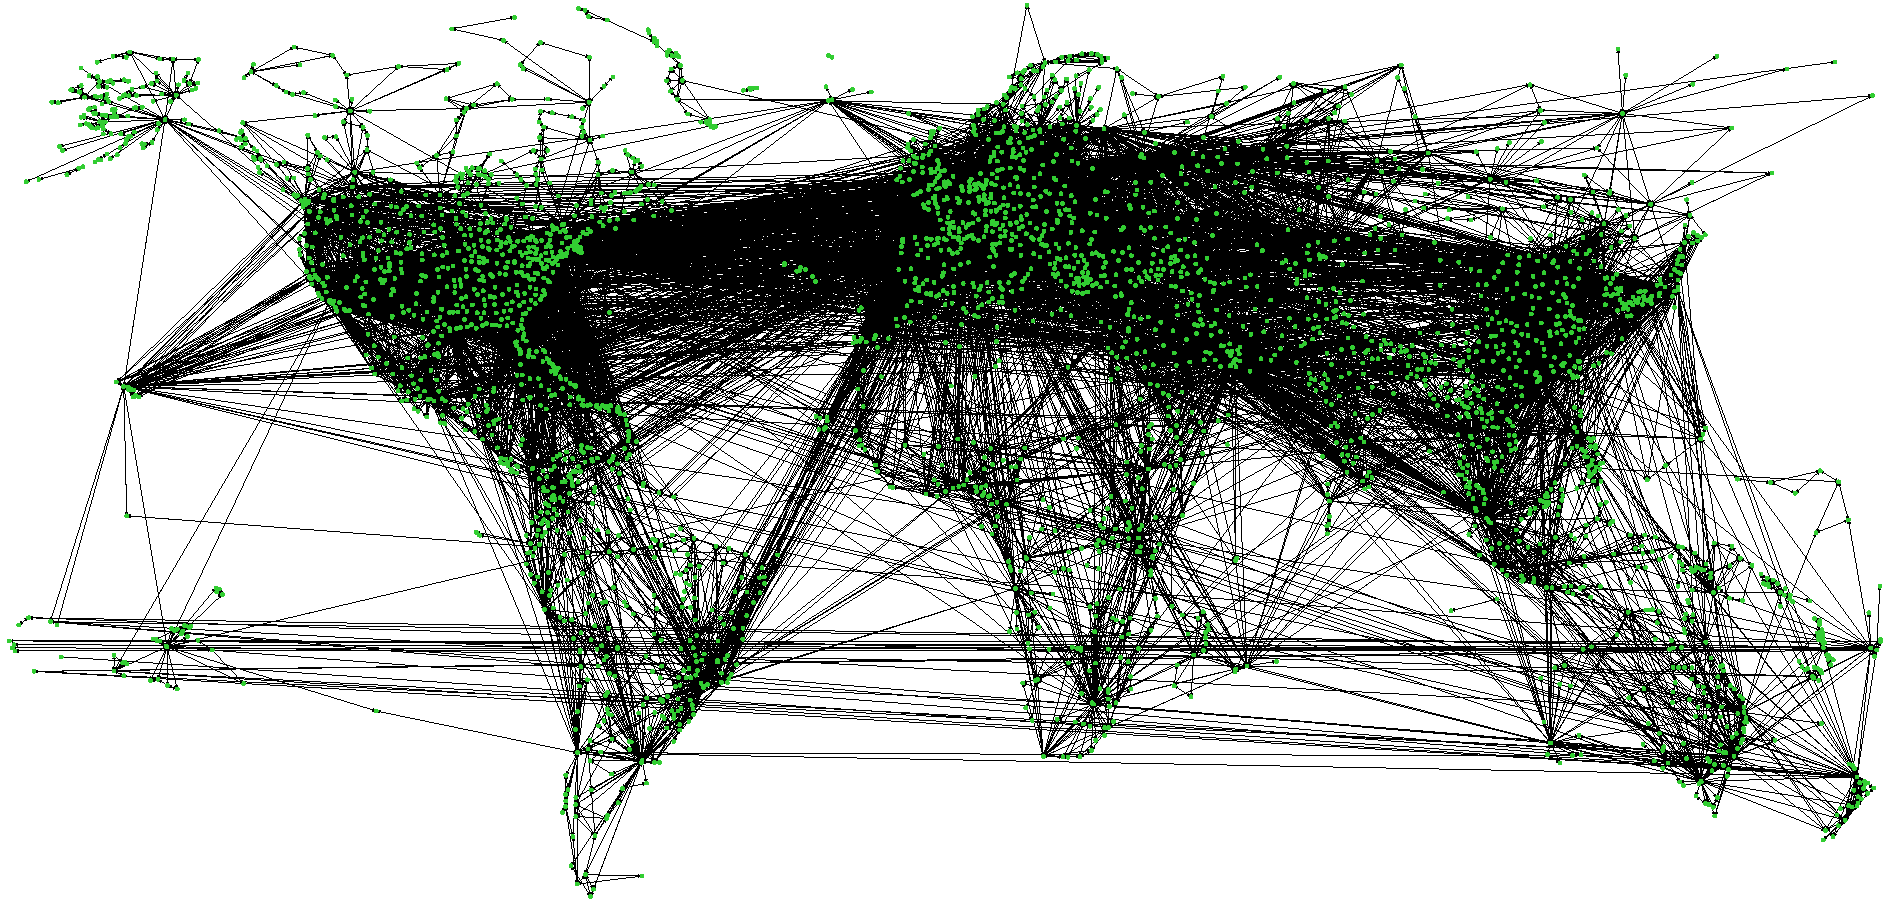
\includegraphics[width=\linewidth]{Figures/final_network.pdf}
    \caption{Visual representation of the flight network covered by our data.}
    \label{fig:final_network}
\end{figure}
%\end{comment}

%%%%%%%%%%%%%%%%%%%%%%%%%%%%%%%%%%%%%%%%%%%%%%%%%%%%%%%%%%%%%%%%%%%%

\subsection{Procedure}
We start by running 100 baseline simulations for a spreading disease using the EoN-Package (Epidemics on Networks) for Python. EoN simulates the spread of a disease in a network by solving an ODE-model (ordinary differential equation) as we have seen it in the class. Furthermore, the specific ODE-model used in this analysis is the SIR-model (susceptible-infected-removed model) which solves three differential equations for each component of the model (S-,I-,R-equation) with respect to t (time-points in the simulation) simultaneously. Through this iterative solving of the equation system we get dynamically rich simulations which are mainly driven by parameters that are specified in the model and the network at hand: Transmission rate of the disease, recovery rate of the people infected, the parameter rho ($\rho$) which sets the number of randomly initial infected entities as a share of the network and the 
$t_max$-parameter, determining the number of periods for which the spread should be simulated. Furthermore, in order to find plausible and consistent findings, the number of iterations for the model has to be set high enough, which depends on the characteristics of the baseline network at hand, meaning the greater the network, the more simulations are needed in order to obtain quasi-consistent solutions for the ODE-model. Since we ran many iterations for the different measures that will be presented later in this part, we decided to use the $fast\_SIR$ in order to keep the computational power needed lower. Otherwise the simulations would have taken much longer to compute, which would decrease our possibilities to test as many simulations as possible in order to obtain significant and robust findings. Furthermore, the $fast\_SIR$ is rather a simple form of the SIR-model since it simulates for exponentially distributed infection and recovery times, which are determined by the user. For a wider analysis of spreading diseases there is a variety of different simulation functions in the EoN package, which allow the user more detailed specifications about the parameters, such as inserting functions for the transmission instead of a singular rate. For the purpose of generality and simplicity we decided to analyze the airport network using only the most simple SIR-model. Furthermore, implementing the much more complicated simulations would go far beyond the scope of this work without adding substantial contribution to the main question of this analysis.  

One crucial problem we had in the beginning was that the $fast\_SIR$ simulation returns very inconsistent arrays of time steps and thus, also number of infected nodes. Since we want to align all the simulation for the same metrics, as well as the averages across the metrics, we need the t-steps to be uniform (or at least consistent). Thus, we used linear interpolation with quite small steps (one tenth of t) to recover uniform information on the number of infected nodes for all of our simulations. After this step was accomplished which made further comparisons between the simulations possible, we started to compute the measures for our analysis which are later used to  remove certain nodes according to the measures in order to analyze the paste of the spread. We implemented measures which are broadly used in the field of network science in order to analyze properties of certain networks and thus make a straightforward interpretation possible. The metrics are: Betweenness Centrality, Closeness Centrality, In-Degree Centrality, Out-Degree Centrality and the Eigenvector Centrality. We used these measures to find the highest ranked nodes in the network according to each measure. Then we defined groups of the top 1\% to 12\% nodes of our network, which we removed from the baseline network in order to analyze the effect of these protective measures on the length of the pandemic and the number of infected people, both the total number and the number of infected individuals in the peak of the number of infected. The range of the groups we use in order to analyze the spread is quite huge, since the top 1\% nodes are equivalent to 33 nodes, while the top 12\% nodes are equal to 394 nodes, corresponding to the baseline network which has a total of 3284 nodes. Through this wide range, we aim to identify the different reductions in speed of the spread. After all these steps we finally get to the point, where we run all the simulations. Since we have 12 groups of nodes which are individually removed for each simulation and 5 measures, we created a total of 60 different scenarios of protective measures in order to analyze the dynamics of the pandemic. 
The prior mentioned parameters set for the simulation were chosen quite arbitrary since both, the transmission rater and recovery rate, do not change the dynamics of the simulation in relative, but rather in absolute terms. It can be shown that the parameters do not change the trend of the pandemics, but only either cause more infections in the peak if the transmission rate is ceteris paribus higher, or on the other hand, the length of the pandemic only gets longer if the recovery rate is ceteris paribus higher. Furthermore, as depicted in Figure ??, the ranking of the different measures does not change when the parameters change, which is a crucial core of our analysis, since it makes our findings (at least relative across the different measures) robust for all combinations of the parameters within the simulation. The parameter $t-max$ was chosen in such a way, that the whole course of the pandemics could be tracked when plotted. The other parameters were chosen, as said before, arbitrarily with the transmission rate being set to 0.005 which means that .... and the recovery rate held constant at 0.5, meaning that an infected individual is recovered after 2 days. Furthermore we set the number of iterations to 100 since it gave us consistent randomization without demanding too much computational time. This means, that for each simulation (for example after removing the top 1\% nodes) we ran 600 iterations of the process, 100 for each of the five measures and the baseline model. We stored each of these results in order to plot them, showing the results of the simulations from different angles, such as the evolution until the peak of the epidemic (corresponding to the number of infections), the entirety of the epidemic, the time until it peaked or the epidemic length in total. 





\begin{figure}[!ht]
    \centering
    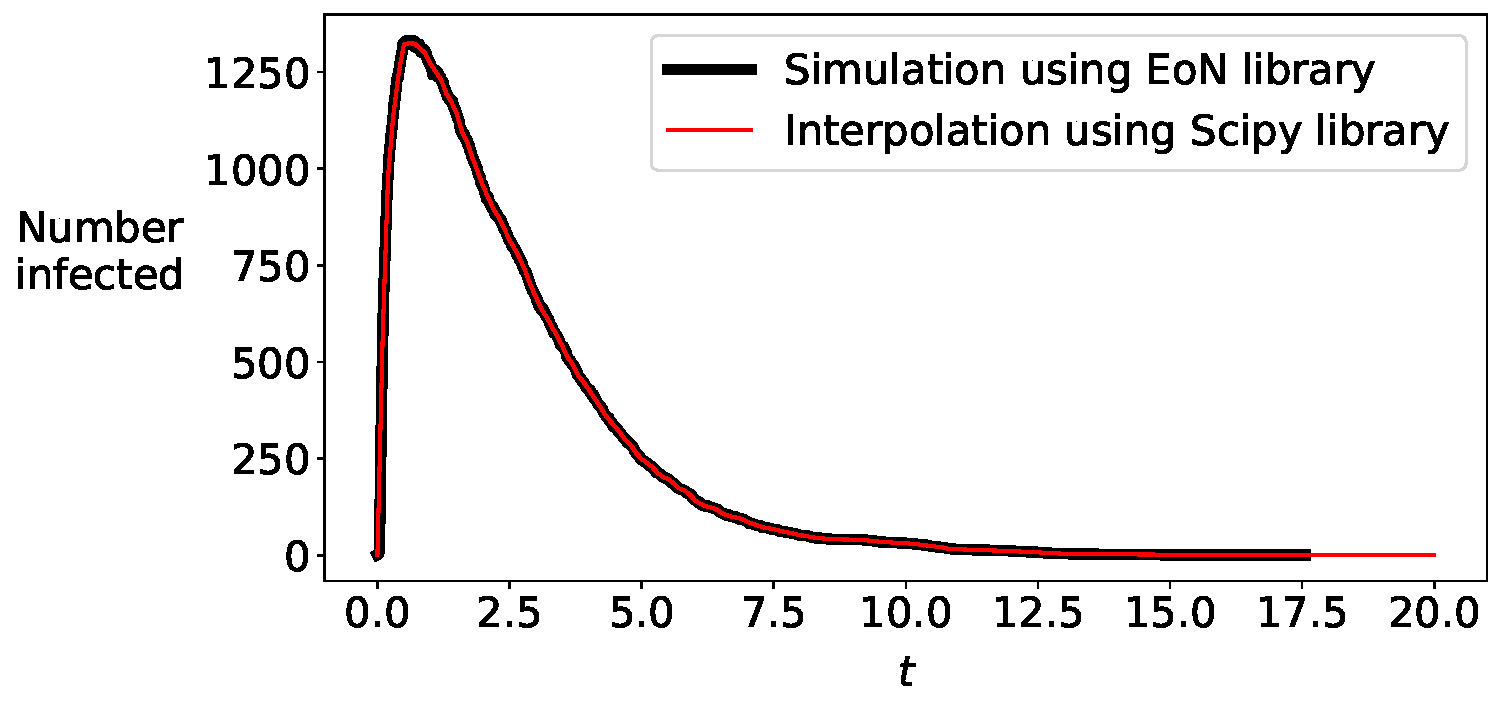
\includegraphics[width=0.5\linewidth]{Figures/interpolation_test.pdf}
    \caption{We use SciPy's \href{https://docs.scipy.org/doc/scipy/reference/interpolate.html}{interpolate subpackage} to reconstruct the simulated epidemic courses since unfortunately our preferred module (\textit{fast\_SIR}) from the EoN library returns very inconsistent arrays of time steps which do not allow us to directly calculate averages and standard errors across multiple simulations. Depicted above is one such example of interpolation. We force infected numbers to be equal to 0 from the moment the epidemic dies until our defined \textit{t-max} parameter (20).}
    \label{fig:interpolation_test}
\end{figure}

%%%%%%%%%%%%%%%%%%%%%%%%%%%%%%%%%%%%%%%%%%%%%%%%%%%%%%%%%%%%%%%%%%%%
%%%%%%%%% RESULTS
%%%%%%%%%%%%%%%%%%%%%%%%%%%%%%%%%%%%%%%%%%%%%%%%%%%%%%%%%%%%%%%%%%%%

\section{Results And Discussion}
In order to study the disease spread of a dynamic global epidemic and to get a picture of the complexity, this requires an analytical representation of the mobility of the air transport network. The scale and complexity of the global air transportation network is evident in Figure \ref{fig:final_network}. As described above, we use the SIR model to simulate the course of an epidemic.

In Figure \ref{fig:interpolation_test} one can observe a graphically example on how we reconstructed the simulated epidemic courses, whereas we used linear interpolation as explained earlier. Here we can observe two important features, one is the peak, i.e. the point with the highest number of infected nodes, secondly the evolution of the SIR simulation over time.
It is evident that the number of infected nodes increases very rapidly and sharply at the beginning of the period, once the epidemic breaks out. However, once we observe more and more nodes that recover, the number of infections fall, but comparatively very slowly and less sharply. 

########Discussion:
In practical comparison, to the Covid-19 pandemic, we could observe similar phenomena, hospitals were often overloaded, because there were very high waves in the outbreak of the infection. This is important to analyze, because seeing how quickly and skyrocketing the disease spreads at the beginning of the outbreak requires decisive policy action. Do we need to close airports faster after the first incident to reduce the likelihood of such a large outbreak, to smooth the emergence of such peaks so that hospitals are not overloaded and more people can be saved?

The experimental design we chose in this study assumes five centrality metrics (betweenness, eigenvector, closeness, in-degree and out-degree centrality) with which popular or in other words, critical airports can be identified. 
In Figure \ref{fig:epidemic_course}, the x\% most critical nodes were shutted off (edges were extracted), which is to simulate a closing of important airports. The goal is to identify how the course of the SIR model would change if we were to simulatively close these central airports. Would the closure of critical airports during an epidemic lead to a relevant change in the course of it?

With the degree centrality method of measuring the importance of a node in a given network, we define that the node with the highest degree, that is, how many connections it has with the other nodes, is more important and therefore has a greater impact on the other nodes. Since this is a directed network where the airports are interconnected depending on the direction of the flight, we considered the indegree and the outdegree. The Indegree is the number of flights arriving and the Outdegree is the number of flights leaving the airport. This means that the most important airports are those that have the most arriving or departing flights to other airports and therefore have a greater impact on the global spread of the disease, as there are more flights to many other airports, with more passengers and therefore a higher probability of infection.
The importance of a node, as measured by Closeness Centrality, is given by how short the distances from it to all others are. Nodes with high Closeness Centrality have the shortest distances to all other nodes and are therefore able to reach other nodes more easily. Thus, the airports with the highest closeness centrality are the main sources of disease transmission, as they spread it very efficiently across the network. This could be the most important centrality measure for our case, since it is a topologically meaningful concept of centrality. The most important airports can easily reach all others, and thus can strongly influence the extent and speed of disease spread across the entire globe.
In the eigenvector centrality method, a node is assigned a relative value with respect to the nodes it is connected to. Thus, the one connected to a node with higher importance always receives a higher centrality value. In this case, it means that the airports connected to an important, i.e. large airport, with many flights (e.g. CDG, Paris Charles de Gaulle, France), are therefore more important than those connected to more unimportant, i.e. smaller airports that do not have many passengers per day (e.g. small airports like on Saba in the Caribbean Islands (SAB)).
In the application of betweenness centrality, all the shortest paths between nodes are taken and observed which node is most visited when traversing the shortest paths, and such a most visited node is the one with the highest centrality or the one with greater importance. That is, an airport with high betweenness centrality may not have the most directed connections with other airports, but if the airports connected to that airport are strongly connected to others, then that airport has high betweenness centrality because there is no other airport that is better positioned in the network. Thus, these airports actually have a great deal of control over the flow of passengers through the network and serve as a bottleneck. They are like a bridge between other airports that are highly interconnected. Thus, the global spread of a disease could be limited by closing such an airport. Because these airports provide a pathway to airports that are otherwise inaccessible, this has a global impact on the entire network. However, local spread of disease in groups connected by that airport may continue to thrive. This measure should be taken with a grain of salt, however, because in real life a flow does not always take the shortest path, which means that the global spread of the disease may not have such a high peak, but may spread slowly globally, but locally there may still be large spreads. But for our focus on global spread, it's an important measure. Second, a bridge may also be at the periphery of the network, and this centrality is also sensitive to changes in the network.

In addition, an interesting insight would be whether the different centrality measures are more likely to identify different airports as important or similar ones. Represented by the matrix of Spearman's rank correlation coefficient between the five selected centrality measures (see Figure \ref{fig:spearman_matrix}). It can be seen that the proximity and eigenvector centrality measures yield very similar rankings of the nodes in our network. The same is true for the in-degree and out-degree centrality measures.

The baseline model in Figure \ref{fig:epidemic_course} simulates the course of the epidemic with all nodes included, i.e. during normal operation of the airports. A steep increase can be seen at the beginning, with infected cases shooting up to 1250 within a short period of time, from where individual nodes start to recover and the curve slowly flattens out until it converges to zero after more than ten times the time. (from t=20 on the value is fixed at 0).
We can see that when only 1\% of the key airports are closed, the course remains very similar to the baseline path. However, the more important airports are closed, the less sharply the number of infected airports shoots up and the course of the epidemic thus has a smoother course. Whereas we can hardly notice a change in the trend of the curve after the top 10\% most important nodes are excluded, this is the case because our network is scale-free, i.e. our netwtwork follows a powerlaw distribution. This means that 
there are a few important airports that have a great influence on the course of the outbreak, since they have the most connections with other airports and are therefore crucial.


It is also noticeable that from the extraction of the 9\% indegree and outdegree most central nodes, the curve becomes nearly flat, there is no increase in infected cases, the cases remain at around 0. In contrast to the betweenness, closeness and eigenvector centrality which still shows a peak of infected cases, but this peak also becomes smaller and smaller, until it hardly changes from 10\%. Compared to the baseline model, the peak is much smaller and has been reduced to about 80\%. In addition, the increase in infected cases is not as sharp at the beginning of the epidemic, the slope of the curve is flatter. Yet the recovery is also slower. To examine these three centrality measures in more depth, it can be seen that the slope of the curve is approximately the same for all of them at the beginning, with the peak being shallowest for closeness centrality and highest for eigenvector centrality. The fall of the infected is slower for the closeness centrality and more drastic for the eigenvector and betweeness centrality, whereby for the latter the recovery process occurs earlier and more strongly and undercuts the closeness centrality in this measure already early, despite the latter’s smaller peak.



In a further step, in Figure \ref{fig:interest_outcomes} we want to take a stronger look at the effects of our outcomes of interest. Shown are the effects of shutting down selected nodes, as discussed earlier, by removing edges on four different outcomes of interest, namely peak of epidemic, entirety of epidemic (how many infected cases there were in total), time until peak, and epidemic length.
Examining the peaks of epidemic, we see that at the baseline model, 40\%  of infected cases were reached only at their peak. By looking at the centrality measures removing the top 1\% most central nodes, between 30 and 40\%  of total nodes were infected at the peak. We see a sharp drop in the rate of infected nodes as more important nodes are removed. Whereas for a removal of 12\%  of the top nodes we reach a rate of infected nodes at the peak below 10\%  for all centrality measures, for the degree centralities even down to almost 0\%. It is remarkable that the BC and CC reach a smaller peak than the degree centralities up to a distance of 6\%  of the nodes, but after that a much flatter course can be observed and thus take on values more like those of the EC, while the degree centralities continue to drop sharply in their height of the peak.
Looking at the entirety of epidemic, we can note that the base model records 70\% infected nodes. Again, we see a very similar trend of the infection rate as before as more important nodes are removed, with the number of infected nodes dropping to below 20\%.  However, a much steeper drop is noted here.
In the third graph, we are interested in how quickly the infected peak is reached. Starting from the baseline model, we notice that we reach the peak within a rapid speed, as the infected nodes are skyrocketing. From the baseline model we can observe a minimal increasing trend up to about 5\% the more important nodes are removed, i.e. the cases of infection increase in a slower pace so to reach the peak it takes longer. Whereas the degree centralities are an exception, the time to peak slows down drastically, by about twice the time compared to the other measures at a removal of 8\% of the most important nodes, but drops from there on to similar values as the other centrality measures.
Last but not least we considered the length of the epidemic, starting from the baseline model we see an overall slightly decreasing trend towards an increase of the top \% of network shut downs. However, the eigenvector centrality shows a fairly constant trend, i.e. there is hardly any change. For the BC and CC we see that the length of the epidemic course is somewhat reduced. The degree centralities are a special case, which is related to the time to peak observations. First, the epidemic length increases until the 7\% of the most important nodes are reduced, followed by a very strong reduction of the length as more nodes are extracted, finally reaching the shortest length of the epidemic course.

It is hard to judge the results above without knowing how similar this topX\% sets are among the different centrality measures. Is the effect of in-degree and out-degree measures almost identical by chance or because we are in fact shutting down the same nodes? Figure \ref{fig:spearman_matrix} already may give us an intuition for what the answer is but it may also throw us off. We calculate a weighted (by the number of nodes being removed) average of the share of nodes that overlap among the topX\% sets of each two measure combination and show the results above. Though the figure seems quite similar to Figure \ref{fig:spearman_matrix} it is noticeable that the eigenvector and closeness correlations are not that high anymore when looking at these two measures from a different angle.





\begin{figure}[!ht]
    \centering
    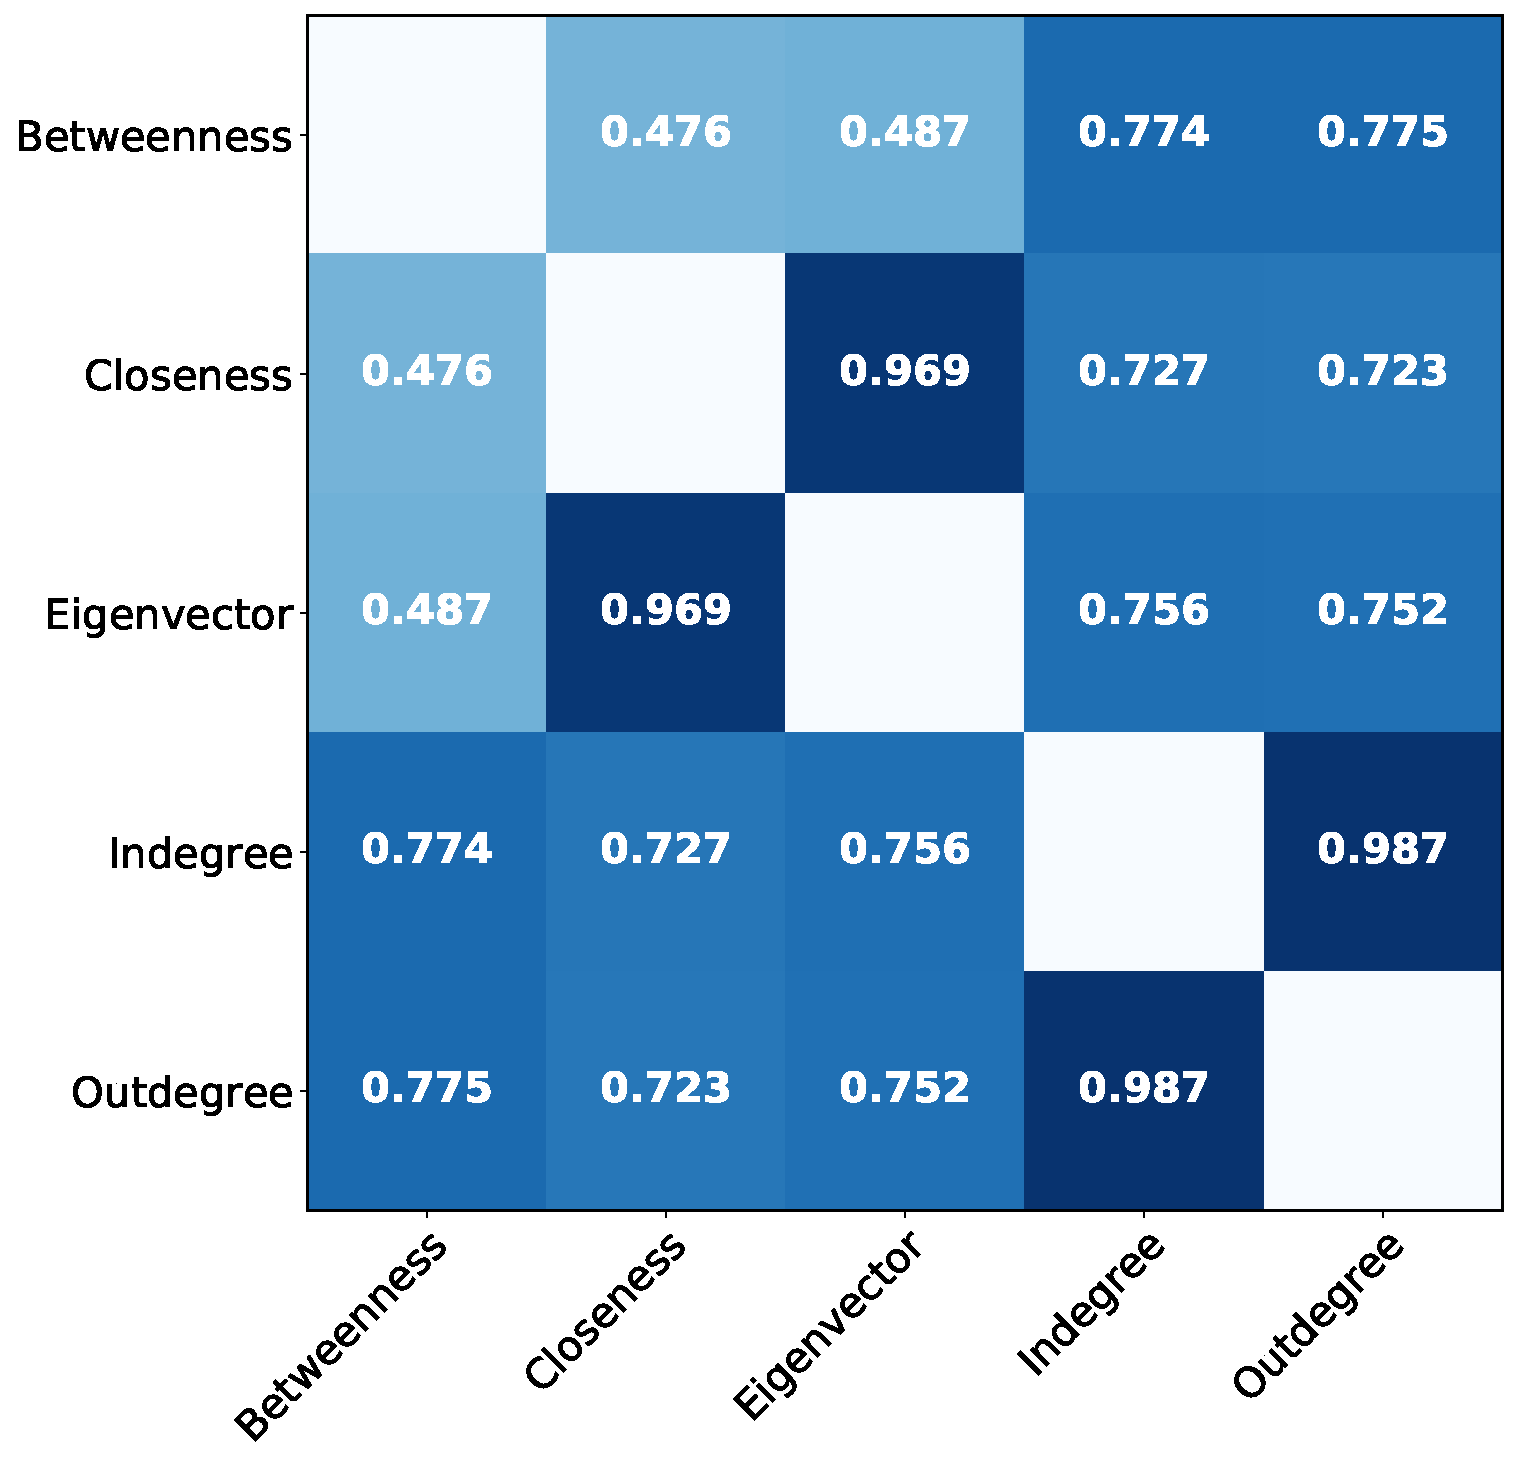
\includegraphics[width=0.5\linewidth]{Figures/spearman_matrix.pdf}
    \caption{Spearman's rank correlation coefficient matrix between the five selected centrality measures. It appears that closeness and eigenvector centrality measures yield an extremely similar ranking of our network's nodes. A similar thing can be seen for the in-degree and out-degree centrality measures.}
    \label{fig:spearman_matrix}  
\end{figure}

\begin{figure}[!ht]
    \centering
    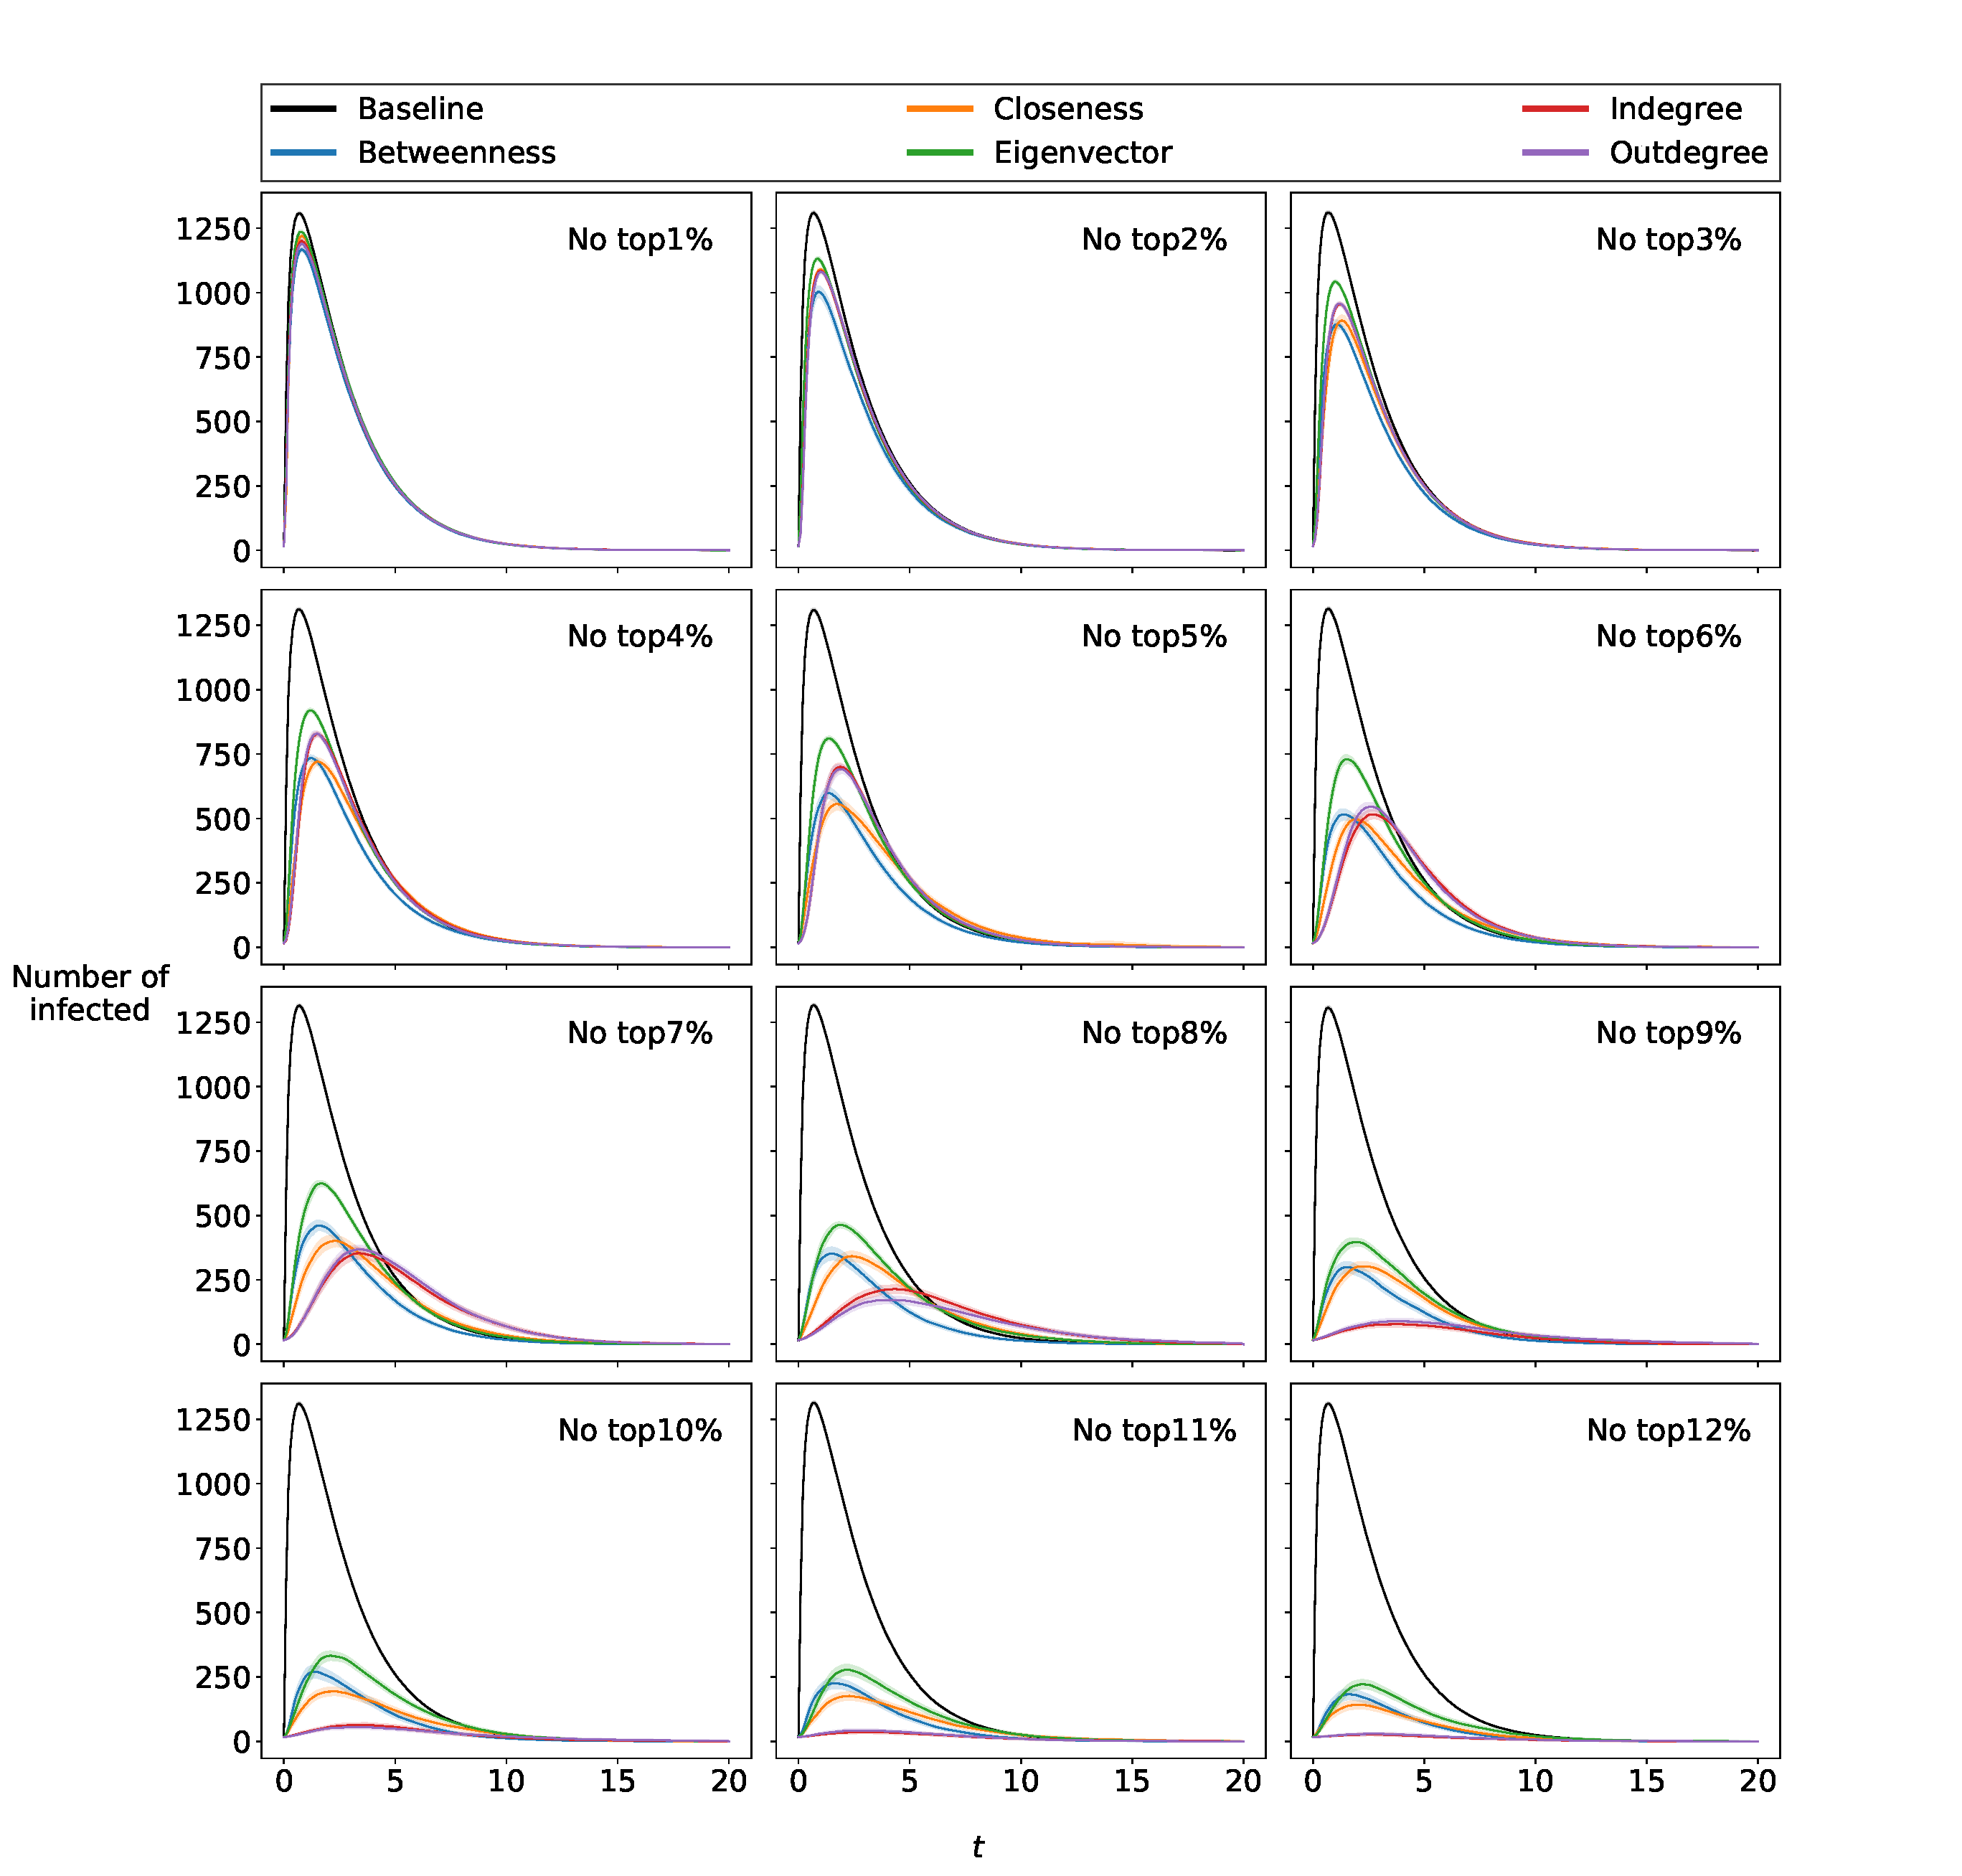
\includegraphics[width=\linewidth]{Figures/epidemic_course.pdf}
    \caption{Depicted are the epidemic courses for the different networks where the top1\% to top12\% highest ranked nodes according to different centrality measures have been shut down (i.e. edges removal). The \textit{baseline} curves are always based on the full network and thus nearly identical (minimal differences are always possible due to the finite nature of the simulation sample). The (almost imperceptible) 95\%-confidence intervals can be seen as halo around the lines.}
    \label{fig:epidemic_course}
\end{figure}

\begin{figure}[!ht]
    \centering
    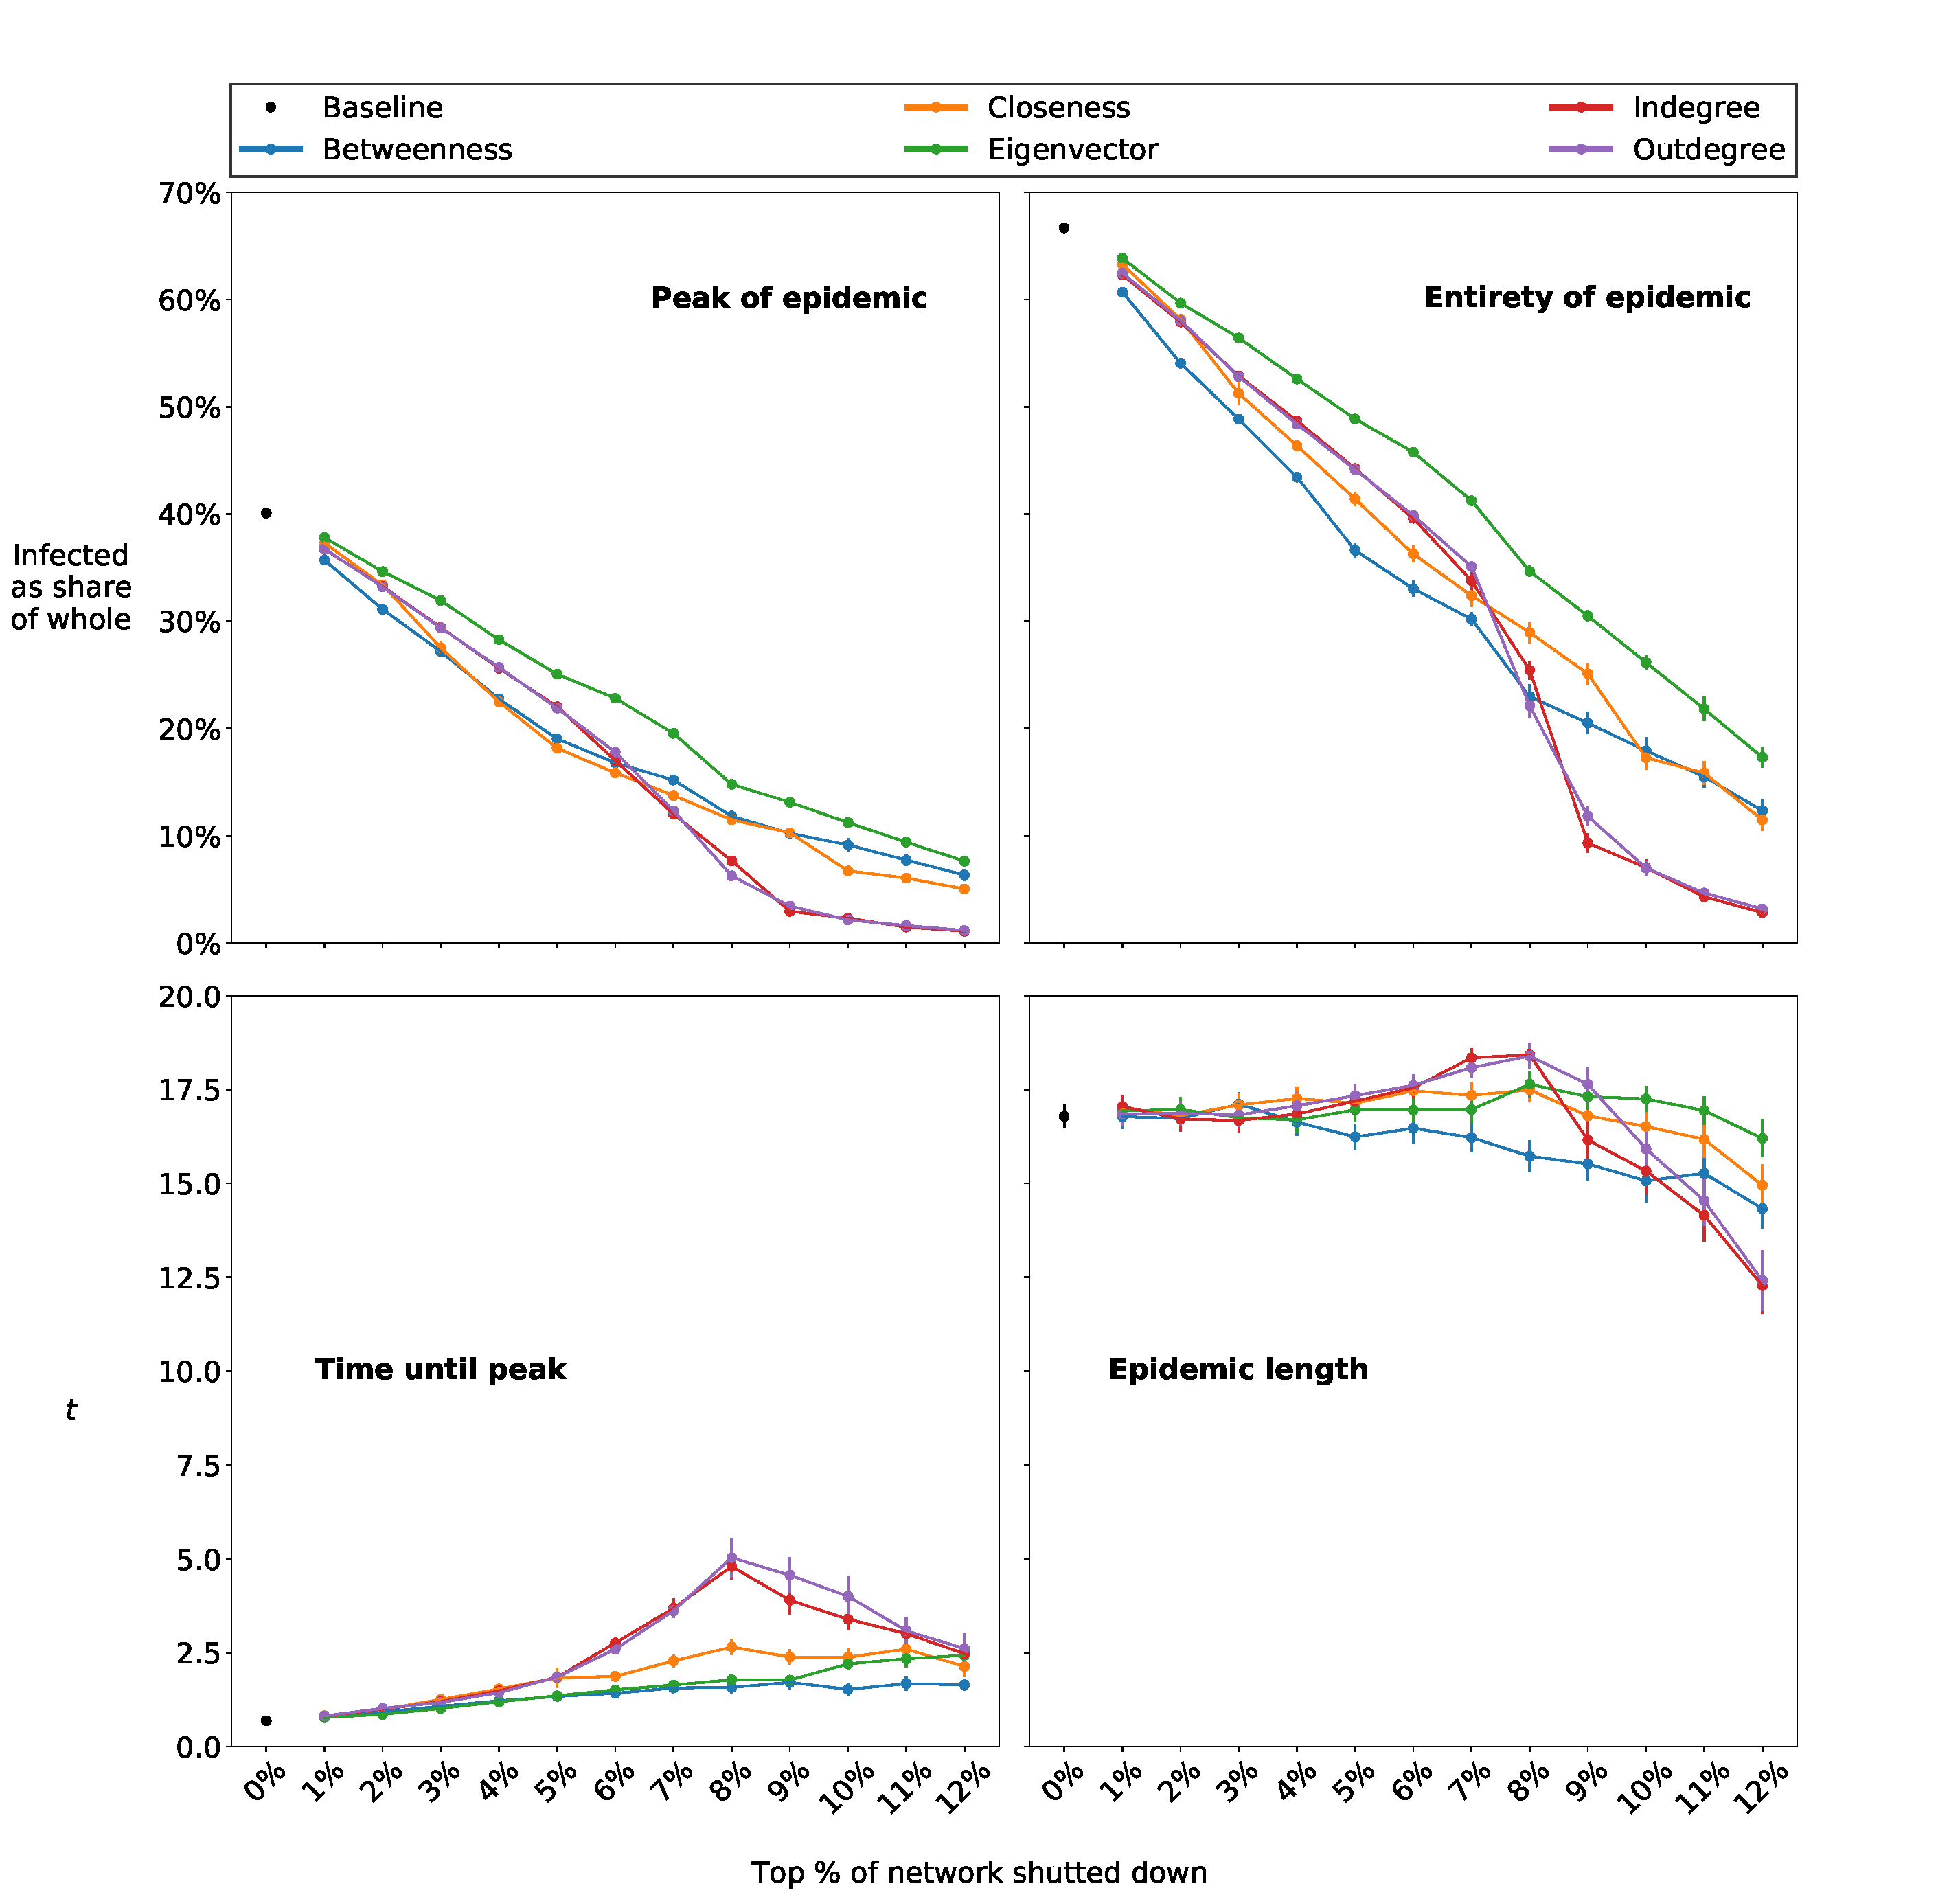
\includegraphics[width=\linewidth]{Figures/interest_outcomes.pdf}
    \caption{Depicted are the effects of selected nodes' shutting down through edges removal on four different outcomes of interest.}
    \label{fig:interest_outcomes}
\end{figure}

\begin{figure}[!ht]
    \centering
    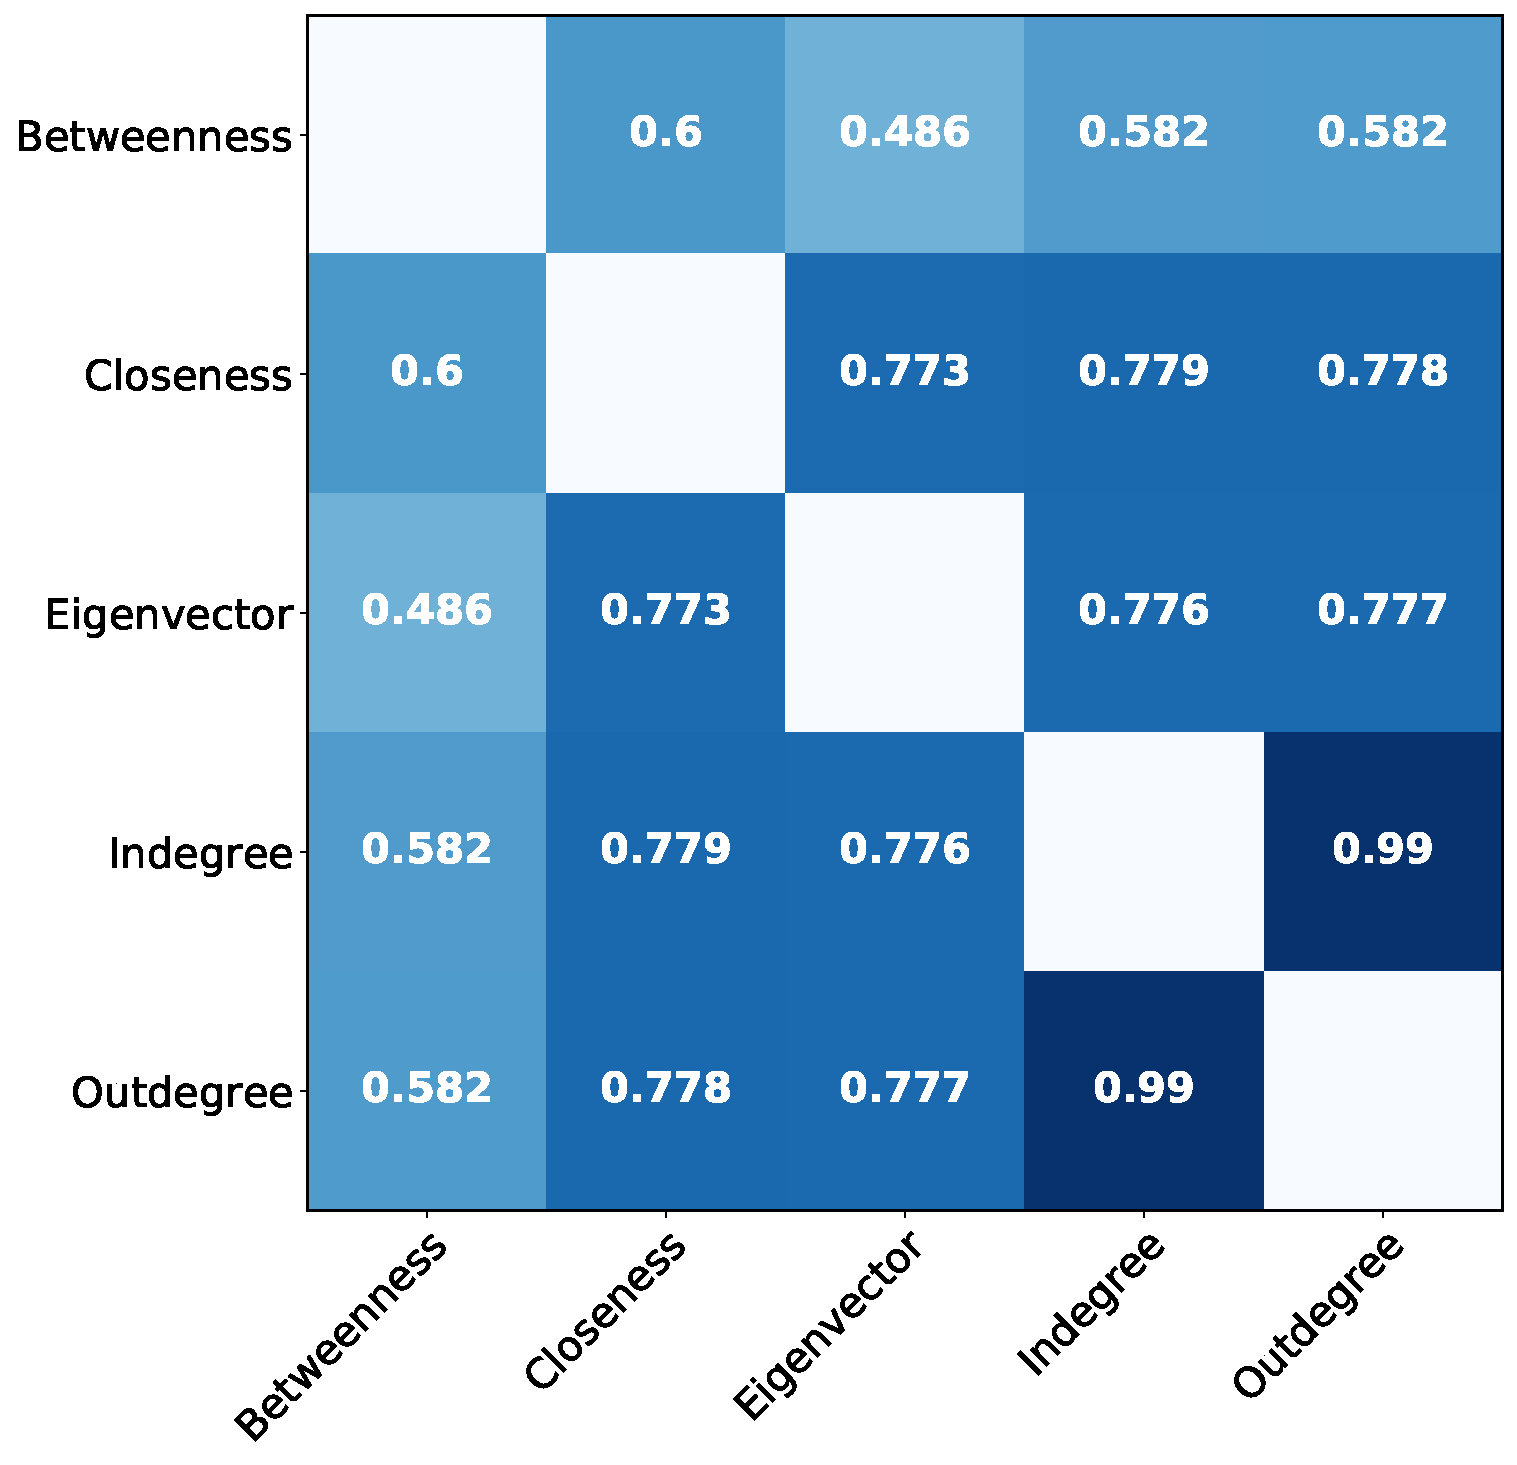
\includegraphics[width=0.5\linewidth]{Figures/node_remove_overlap_matrix.pdf}
    \caption{It is hard to judge the results above without knowing how similar this topX\% sets are among the different centrality measures. Is the effect of in-degree and out-degree measures almost identical by chance or because we are in fact shutting down the same nodes? Figure \ref{fig:spearman_matrix} already may give us an intuition for what the answer is but it may also throw us off. We calculate a weighted (by the number of nodes being removed) average of the share of nodes that overlap among the topX\% sets of each two measure combination and show the results above. Though the figure seems quite similar to Figure \ref{fig:spearman_matrix} it is noticeable that the eigenvector and closeness correlations are not that high anymore when looking at these two measures from a different angle.}
    \label{fig:node_remove_overlap_matrix}
\end{figure}

%%%%%%%%%%%%%%%%%%%%%%%%%%%%%%%%%%%%%%%%%%%%%%%%%%%%%%%%%%%%%%%%%%%%
%%%%%%%%% DISCUSSION
%%%%%%%%%%%%%%%%%%%%%%%%%%%%%%%%%%%%%%%%%%%%%%%%%%%%%%%%%%%%%%%%%%%%
%\clearpage
%\section{Discussion}
%\subsection{Analysis}
%Here we discuss.

%%%%%%%%%%%%%%%%%%%%%%%%%%%%%%%%%%%%%%%%%%%%%%%%%%%%%%%%%%%%%%%%%%%%
%\clearpage
%\subsection{Validation}
%And here we validate.

%%%%%%%%%%%%%%%%%%%%%%%%%%%%%%%%%%%%%%%%%%%%%%%%%%%%%%%%%%%%%%%%%%%%
%%%%%%%%% CONCLUSION
%%%%%%%%%%%%%%%%%%%%%%%%%%%%%%%%%%%%%%%%%%%%%%%%%%%%%%%%%%%%%%%%%%%%
\clearpage
\section{Conclusion}
Finally, the conclusions. Bye.

%%%%%%%%%%%%%%%%%%%%%%%%%%%%%%%%%%%%%%%%%%%%%%%%%%%%%%%%%%%%%%%%%%%%
%%%%%%%%% REFERENCES
%%%%%%%%%%%%%%%%%%%%%%%%%%%%%%%%%%%%%%%%%%%%%%%%%%%%%%%%%%%%%%%%%%%%

\clearpage
\printbibliography

%%%%%%%%%%%%%%%%%%%%%%%%%%%%%%%%%%%%%%%%%%%%%%%%%%%%%%%%%%%%%%%%%%%%
%%%%%%%%% AUTHOR CONTRIBUTIONS
%%%%%%%%%%%%%%%%%%%%%%%%%%%%%%%%%%%%%%%%%%%%%%%%%%%%%%%%%%%%%%%%%%%%
\newpage
\section*{Author contributions}
All authors conceived and designed the project idea. M. Vázquez prepared and analysed the data, produced figures. All authors revised and accepted the final version of this document.

%All authors conceived and designed the project idea. P.M. and C.J.T. performed the literature review and wrote the introduction. B.S. performed the data collection. Y.Z. and X.Y. analysed the data. B.S. wrote the bulk of the text. All authors discussed and reached the conclusions. All authors revised and accepted the final version of this document.

\end{document}

